\documentclass{report}
\usepackage[a4paper, margin=0.5in]{geometry}
\usepackage{parskip}
\usepackage{graphicx}
\usepackage{caption}
\usepackage{amssymb}
\usepackage{amsmath}
\usepackage{algpseudocode}
\usepackage{algorithm}

\captionsetup[figure]{
  font = it,
  labelfont = bf
}

\begin{document}
\begin{minipage}[b]{0.48\textwidth}
  \section*{Hamerly's Algorithm}
  Hamerly's algorithm is an optimization of the standard algorithm and takes advantage of the fact that it is not necessary to recalculate the distance of each point from the centroids each time the centroids are repositioned. Using the \textbf{triangular inequality} it is, in fact, possible to identify critical points, that is, points for which it is necessary to recalculate the distance to each centroid to find the closest one. In contrast, for the other points, the class to which they were assigned remains the right one even if the centroid has been moved.

  \section*{Triangular inequality}
  Given 3 points A, B, C $\in \mathbb{R}^2$ then  
  \begin{equation}
      d(A, B) \leq d(A, C) + d(B, C)
  \end{equation}
  \begin{equation}
      d(A, C) \leq d(A, B) + d(C, B)
  \end{equation}
  \begin{equation}
      d(C, B) \leq d(C, A) + d(B, A)
  \end{equation}
  Where $d(\alpha, \beta)$ is the distance between the points $\alpha$ and $\beta$.

  That is, the distance between any two points is less than the sum of the distances between the first point and the third and the second point always with the third one.

  This inequality can also be interpreted geometrically: referring to Figure \ref{fig:triineq}, any one side of a triangle is definitely less than or equal to the sum of the other two sides.

  \hspace{0.1in}
  \begin{center}
    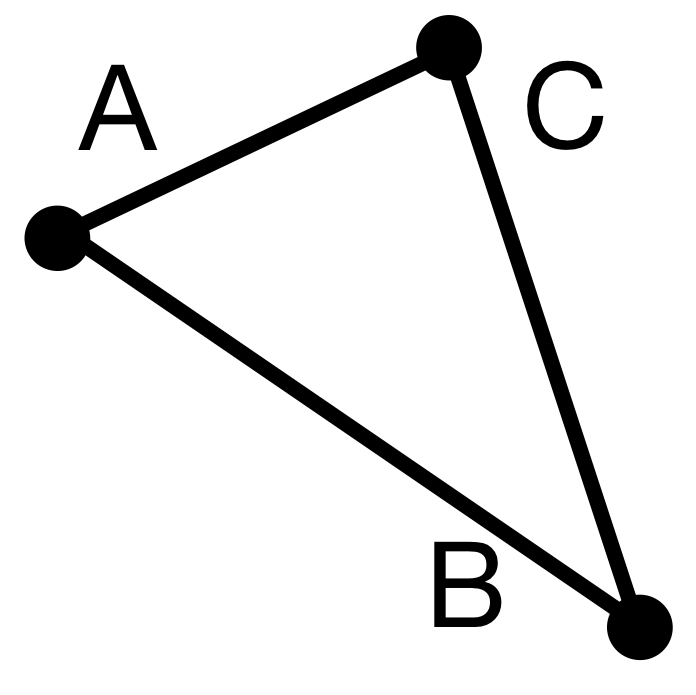
\includegraphics[width = 0.25\textwidth]{imgs/triangle.png}
    \captionof{figure}{3 points in space forming a triangle}
    \label{fig:triineq}
  \end{center}

  \subsubsection*{Disuguaglianza triangolare e k-means}
  For simplicity, let us assume that we have only one point and two centroids (Figure \ref{fig:triCC}).  

  \begin{center}
      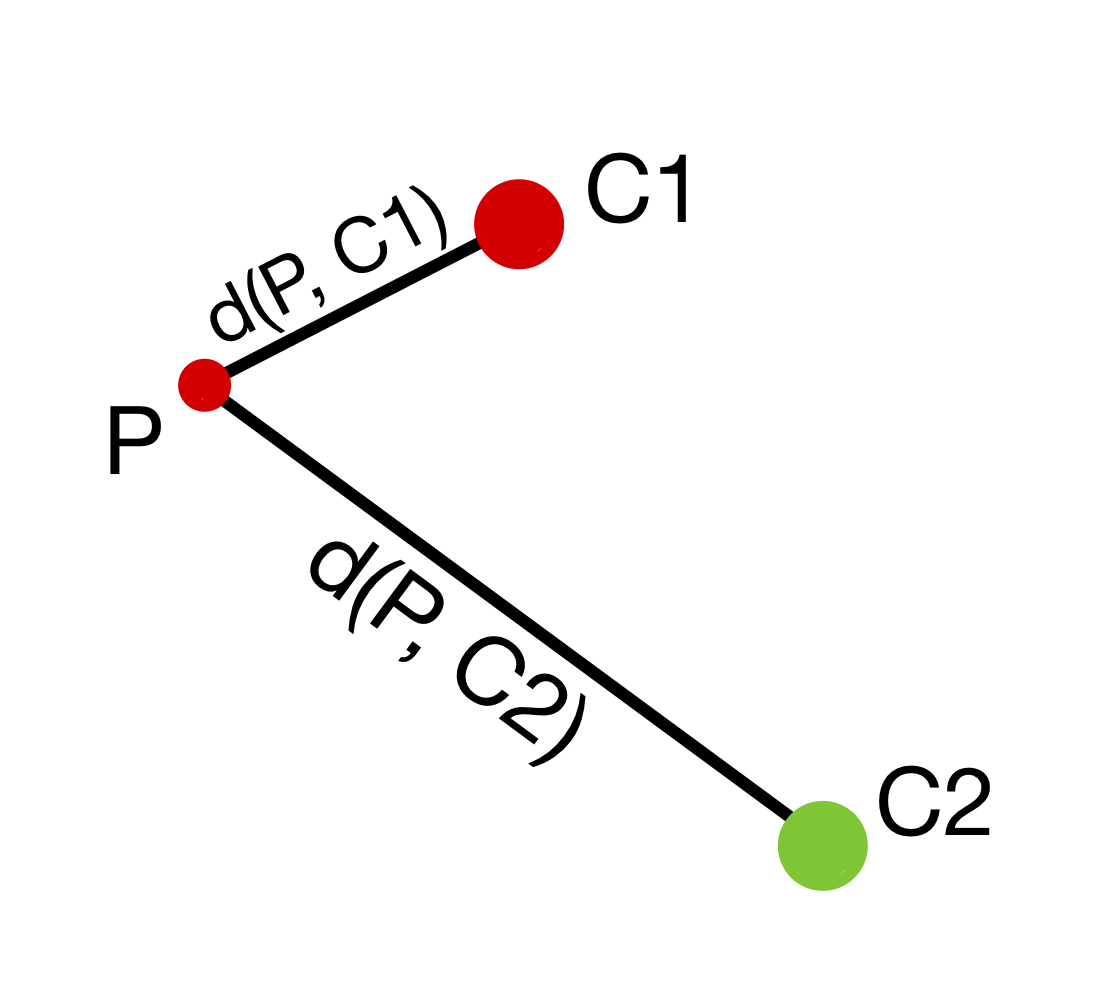
\includegraphics[width = 0.45\textwidth]{imgs/triCC.png}
      \captionof{figure}{Example with 2 centroids and one point}
      \label{fig:triCC}
  \end{center}

  At this point we assume that the centroids shift (Figure \ref{fig:triCCafter}), because of the other points (which are not represented).

  \begin{center}
      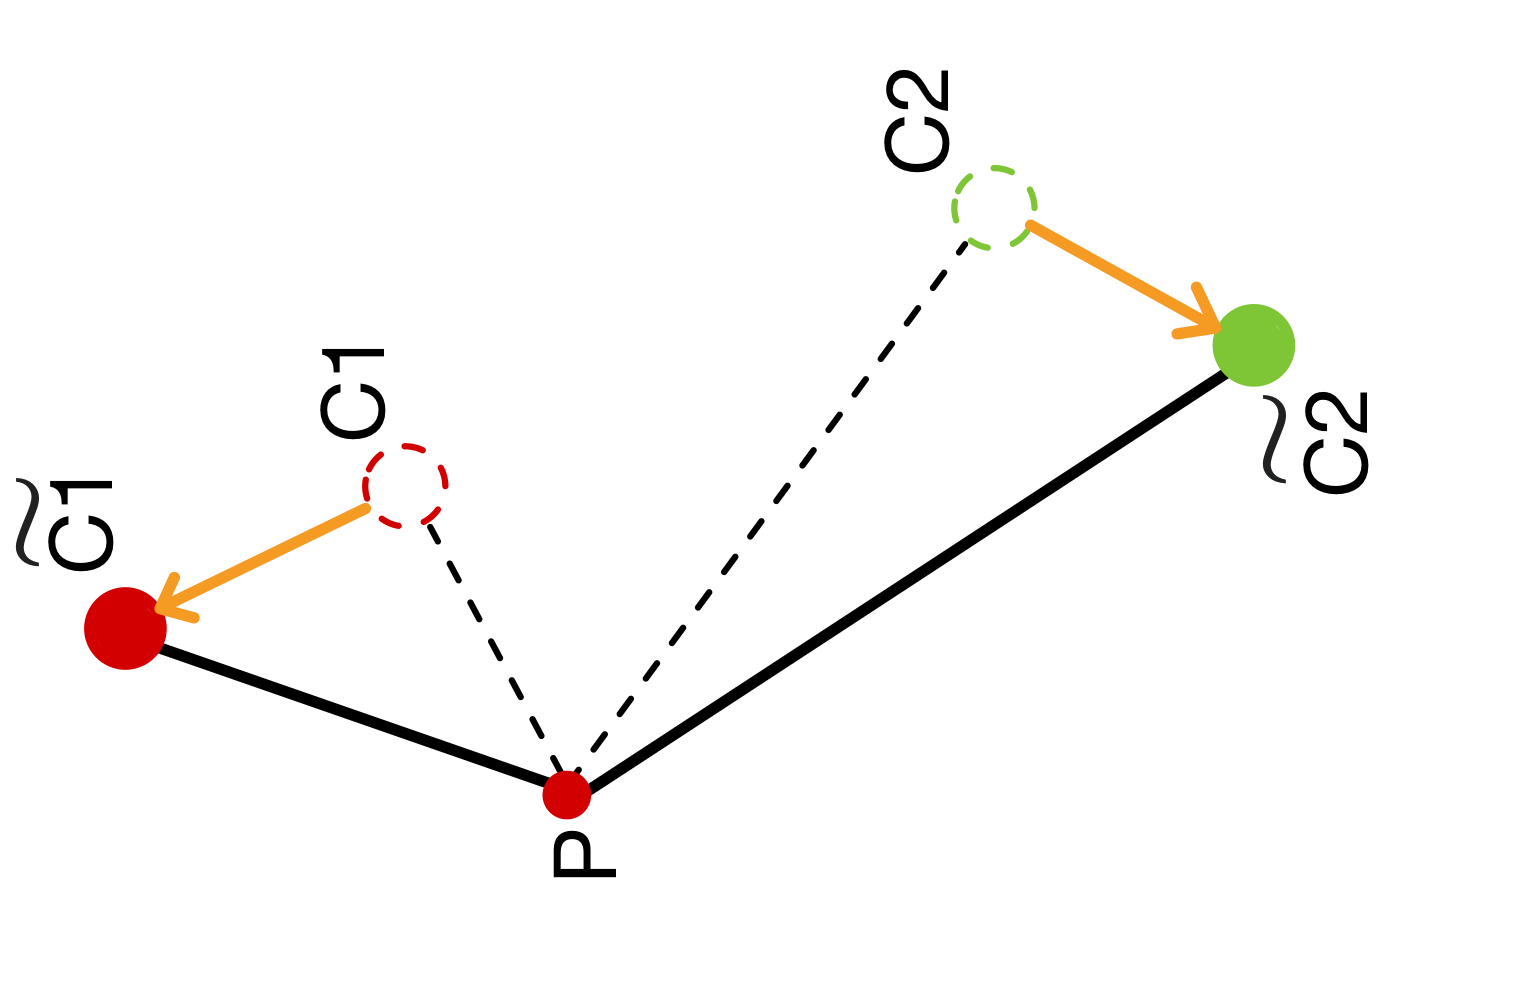
\includegraphics[width = 0.6\textwidth]{imgs/triCCAfter.png}
      \captionof{figure}{Example after the centroids have shifted}
      \label{fig:triCCafter}
  \end{center}   
\end{minipage}
\hspace{0.1in}
\begin{minipage}[b]{0.48\textwidth}
  Thanks to the triangular inequality, we can state that the distance between P and $\tilde{C_1}$ is:
  \begin{equation}
      d(P, \tilde{C_1}) \leq d(P, C_1) + d(C_1, \tilde{C_1})
  \end{equation}
  And in the same way:
  \begin{equation}
    d(P, \tilde{C_2}) \leq d(P, C_2) + d(C_2, \tilde{C_2})
  \end{equation}

  In words, we can say that the distance between point P and one of the centroids is definitely less than the old distance plus the distance traveled by the centroid.

  Taking advantage of this result, we can improve the k-means algorithm as described s follow.
  The first step remains mostly unchanged: it consists of assigning to each point the nearest centroid, and to do this it is necessary to calculate all the distances between the point and the centroids. The difference with the standard algorithm is that in this case, for each point, we have to save the distance ($\mu$) to the nearest centroid and also the distance (l) to the second nearest centroid.

  Assuming, for example, that for a point (P), the nearest centroid is $C_1$ we have that
  \begin{equation}
      \mu = d(P, C_1)
  \end{equation}
  \begin{equation}
      l = \min\limits_{C_i \neq C_1} d(P, C_i)
  \end{equation}

  After the first step, the centroids are repositioned and again the algorithm is almost identical: eqs 2 and 3 are used to compute the new position of the centroids, but unlike before, the distance ($d_i$) traveled by the i-th centroid, the distance traveled by the centroid that moved the most ($d_1^{max}$) and the distance traveled by the second centroid that moved the most ($d_2^{max}$) are also saved.

  At this point, the parameters $\mu$ and l are updated for each point, as follows.

  \begin{equation}
    \tilde{\mu} =  \mu + d_i
  \end{equation}
  If the closest centroid is also the one that moved the most then.
  \begin{equation}
      \tilde{l} = l - d_2^{max}
  \end{equation}
  Altrimenti
  \begin{equation}
      \tilde{l} = l - d_1^{max}
  \end{equation}

  These updates are justified by the triangular inequation. In fact, we know that after the centroids have moved, the point cannot be farther than $\tilde{mu}$ from the nearest centroid and at the same time cannot be closer than $\tilde{l}$ from the second nearest one.

  Thanks to the previous step, it is possible to identify as \textbf{critical the points for which } $\mathbf{\tilde{mu} \geq \tilde{l}}$, that is, the points for which the assigned centroid may not be the nearest
  
  The next step is, then, to iterate for all points but recalculating the distance to the nearest centroid only for the critical ones. Moreover, we can optimize this process even more since, once a critical point has been found, it may be sufficient to recalculate only $\tilde{\mu}$, i.e., the distance to the nearest centroid, and then recheck the condition $\tilde{mu} \geq \tilde{l}$ and only if the condition is still verified then it will be necessary to carry out the full calculation of the distances.
  
  Finally, the centroids are repositioned and the procedure is repeated until the condition of convergence is reached.
\end{minipage}

\newpage

\begin{minipage}[b]{0.48\textwidth}
  \section*{Number of iterations}
  In the case of Hamerly's algorithm, the number of iterations required to complete the classification is:
  \begin{equation}
      kN_cN_p + mk(\phi N_pN_c + (1 - \phi)N_p)
  \end{equation}
  Where $\phi$ is the percentage of critical points to the total number of points.

  The improvement over the standard algorithm lies in the fact that only the first time it is necessary to compute all distances, whereas in subsequent iterations, for most points, there is no need to recompute the nearest centroid.

  \section*{Parallelize the Hamerly's algorithm}
  The Hamerly's algorithm has three main sub-tasks: assignation of the points to a class, update of the centroids, update the lower and upper bounds of all points.

  \subsubsection*{Assignation of the points to a class}
  In this phase, each point will be assigned to a centroid which will represent its class. If it is the first iteration, this can be easly parallelizable by simply partitioning the points between the threads. Each thread will then goes through its set of points and find the minimum distance between the point and the centroids and therefore will assign to point to that class. In this first ieration the work load is equally balanced across the threads because the work that has to be done for each point is the same.

  This is not true from the second iteration, because in this case the only points for which the minimum distance is calculated are the critical points. Therefore it is not enough to partion the points between the threads because criticals points could be not equally distribuited across the point set and because of this some threads could have more work to do compared to others. A load balancing tequiniche has to be used.

  Whatever the iteration, another important task is done during this phase: tracking the points assigned to a class. Suppose for example that we have 3 class and the dimensionality of the data is 2, then one of the private paramenter of the hamerly class will be a 3x2 matrix (called average\_per\_class) and an array with a length of three (called points\_per\_class). The first one tracks, for each class (average\_per\_class[i]) the sum of all coordinates of the points that, during this phase, have been assigned to the i-th class. The points\_per\_class instead track the number of points assigned to each class. Notice that when a point is assigned to a class (say the i-th class), its coordnate are added respectively added to average\_per\_class[i][0] and average\_per\_class[i][1] but if the point was previously assigned to another class, its coordinates have to be removed from the previous class.

  \subsubsection*{Update of the centroids}
  This is the phase where the centroids are moved. Also this step can be easly parallized by simply partitioning the centroids between the threads which, for every of its centroid will divide the sum of all coordinates of the points assigned to that class by the number of points. These information are saved in the average\_per\_class matrix and the points\_per\_class array.
\end{minipage}
\hspace{0.1in}
\raisebox{8in}{
\begin{minipage}[b]{0.48\textwidth}
  The work load for every centroid is the same, therefore no special cautions are needed when parallelizing it.
  During this step, we must also save the distances taken by each centroid (in an array called cdistaces), the maximum distance taken from the centroid (in a variable maxdist) and its index (maxdist\_index), the second maximum distance taken from the centroids.

  \subsubsection*{Update the lower and upper bounds of all points}
  During this step, the lower and upper bound of each points are updated using the information saved during the "Update of the centroids". This is where the balancing algorithm is applied and the result of this phase is an array (called criticals) containing the address of all critical points that have been found. 
\end{minipage}}
\end{document}